\documentclass[conference]{IEEEtran}
\usepackage{cite}
\usepackage[portuges,brazil]{babel}
\usepackage{amsmath,amssymb,amsfonts}
\usepackage{siunitx}
\usepackage{algorithmic}
\usepackage{graphicx}
\usepackage{textcomp}
\usepackage{hyperref}
\usepackage{listings}
\usepackage[toc,page]{appendix}
\usepackage[utf8]{inputenc}

\def\BibTeX{{\rm B\kern-.05em{\sc i\kern-.025em b}\kern-.08em
    T\kern-.1667em\lower.7ex\hbox{E}\kern-.125emX}}

\begin{document}

\title{Projeto 4: Esteganografia\\
\large .\\
\large MC920 - Introdução ao Processamento Digital de Imagem (MC920 / MO443) 2S2019\\
\large Professor: Hélio Pedrini}

\newcommand{\email}[1]{\href{mailto:#1}{#1}}

\author{
    \IEEEauthorblockN{Giovani Nascimento Pereira}
    \IEEEauthorblockA{
    \email{giovani.x.pereira@gmail.com} \\
    168609
    }
}

\maketitle

\section{Definição do problema}

    Esteganografia é uma forma de transmissão de dados codificados em imagens.

    \subsection{Objetivo}

        O objetivo deste trabalho é de implementar métodos de esteganografia, codificando mensagens em imagens e depois sendo capaz de recuperá-las.

    \subsection{Execução do projeto}

        Para executar os projeto, existem 2 scripts:

        \begin{itemize}
            \item codificar.py
            \item decodificar.py
        \end{itemize}

        Para executar os scripts são utilizados os comandos:


        Onde \textit{input$\_$image} é o caminho da imagem de entrada, na qual será codificada a mensagem.
        \textit{input$\_$text} é o caminho do texto a ser codificado.
        \textit{output$\_$text} é o caminho do texto de saída gerado na decodificação.
        \textit{bits} é qual bit menos significativo será alterado para a codificação da mensagem.
        E onde \textit{output$\_$image} é o caminho da imagem gerada na codificação.

        A única \textit{flag} disponível para a execução é a \textit{-d} que habilita que informação de debug seja imprimida na saída padrão.
        Isso inclui etapas intermediárias do processo de conversão de caracteres em uma string binárias para a codificação e do processo reverso também.

\section {Codificação}

    \subsection{Conversão do texto em binário}

    Para ser inserido na imagem, o texto de entrada deve ser convertido em uma sequência de bits que representa o mesmo texto.
    Isso foi feito, para cada caracter, convertendo para seu valor na tabela ASCII. Com esse valor numérico, ele foi transformado numa string que representava o mesmo valor mas em codificação binária.

    Por exemplo, o caracter $a$, equivale a $97$ na tabela ASCII.
    Com esse valor, convertemos $97$ em binário $01100001$.

    É importante que as strings que representam os caracteres tenham exatamente $8$ caracteres, isso garante consistência no nosso processo e facilita a decodificação.

    Esse processo é repetido para todo caracter do texto de entrada, e concatenado com o texto em binário final a ser codificado.

    Ao final, também foi adicionado um caracter que não pertencia ao texto de entrada, chamado de \textit{caracter de parada}. Este caracter é uma sequência de 8 zeros $00000000$. Na tabela ASCII este caracter de valor $0$ não representa um caracter visível, e no nosso caso, pode ser usado para demarcar o fim do arquivo a ser lido.

    Caso não houvesse um caracter de parada, ficaria mais difícil definir durante a decodificação quando a mensagem teria acabado, podendo tentar decodificar a imagem toda durante o processo e não apenas a parte que contém a mensagem desejada.

    \subsection{Codificação na imagem}

    Para inserir a mensagem, já representada em uma string binária, na imagem, é iterado sobre a imagem pixel a pixel e em cada canal de cor RGB da mesma (nessa ordem), modificando o bit menos significativo escolhido com o valor da string desejada.

    Por exemplo próximo valor a ser inserido é $1$ no bit menos significativo, e a imagem tem um pixel preto, que indica que todo canal de cor RGB tem valor mínimo, zero.
    Então o valor do pixel, representado em binário é $00000000$, adicionando o valor desejado tem-se $00000001$.

    E este processo é repetido para todos os caracteres da mensagem a ser codificada.


\section {Decodificação}

    \subsection{Leitura da Imagem}

    A imagem é aberta da mesma forma e o bit no qual a mensagem deve estar codificada é apresentado.

    Com essas informações, a fim de extrair a mensagem da imagem, basta iterar sobre todos os pixels na ordem correta dos canais de cor RBG e ir \textit{acumulando} o valor dos bits menos significativos.

    \subsection{Conversão em texto}

    O acumulado de todos os bits extraídos dos pixels da imagem é a sequência de bits que pode corresponder a mensagem desejada.
    Para descobrir tanto, é iterado sobre esse conjunto de bits de 8 em 8, pois cada caracter é representado em 8 bits.

    Um conjunto de 8 bits representa um valor numérico, então podeos converte-lo em um numero, e depois disso pegar o valor equivalente na tabela ASCII.

    Fazendo esse processo corretamente é possível extrair uma mensgaem que tenha sido codificada na imagem.

    Além disso, esse processo pode parar se o caracter de parada, que tem valor numérico $0$, for encontrado.

\section{Resultados}

    As imagens foram geradas usando um texto de XXXX caracteres.

    Para a imagem do \textit{baboon.png} que tem dimensão X x X, ou seja, contém XXX pixels, colm capacidade


\section{Análises}

    É possível notar quer as imagens finais geradas depois do processo de codificação das mensagens são muito semelhantes às imagens originais.

    Isso se deve pelo fato que os valores modificados na imagens se referem aos bits menos significativos das mesmas, assim as mudanças em níveis de cor são pouco refletidas.
    Isso mesmo até para os textos grandes.

    Contudo, com uma análise mais profunda dos valores dos pixels, é possível notar sim que há uma mudança na cor dos pixels modificados.
    Isso pode ser observado na imagem a seguir:

    \begin{figure}[ht]
        \centering
        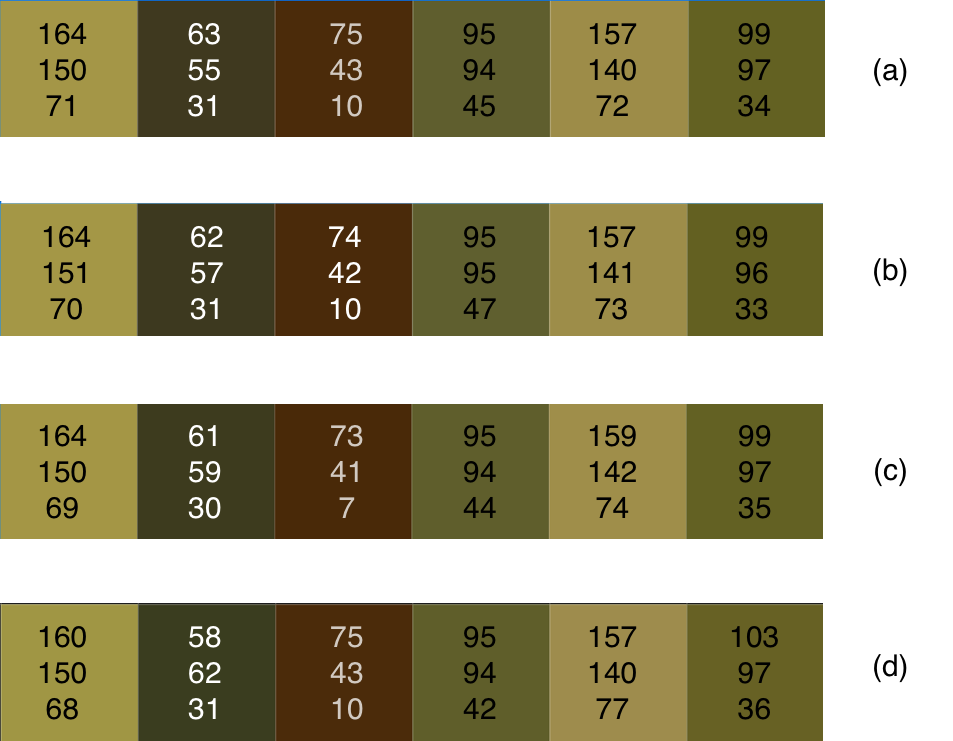
\includegraphics[width=\linewidth]{baboonColors.png}
        \caption{Esquematização dos 6 primeiros pixels da imagem \textit{baboon} com os níveis de cor explicitados em cada pixel, na ordem R G e B. a - Imagem original. b - imagem aplicada esteganografia para o bit menos significativo. c - imagem aplicada esteganografia para o segundo bit menos significativo. d - imagem aplicada esteganografia para o terceioro bit menos significativo}
        \label{fig:bbc}
    \end{figure}

    Mesmo havendo mudanças, elas são sutis, e ao observar a imagem como um tudo não é possível notar diferenças.

    Dessa forma, uma mensagem esteganografada numa imagem colorida é muito difícil de ser percebida, apesar de se tratar de um processo relativamente simples de codificação.

\section{Conclusão}

    Através do resultados obtidos no projeto é possível dizer que o experimento foi satisfatório.
    De maneira geral foi possível codificar mensagens em imagens coloridas (.png) e depois obter as mesmas mensagens através apenas das imagens codificadas.

    AO observar os valroes dos pixels das inagens, foi possível notar que os níveis de cinza foram alterados em seus bits menos significativos (quando observados em valores binários) em relação à imagem original.


\begin{thebibliography}{00}

  \bibitem{helio} Helio Pedrini. Trabalho 4. Introdução ao Processamento Digital de Imagem (MC920 / MO443), 2019.\\

  \bibitem{srgb} SRGB. disponível em \url{https://en.wikipedia.org/wiki/SRGB}. Acesso 11 de setembro de 2019.

\end{thebibliography}

\end{document}
